\begin{refsection}[research/ito/group.bib]
\nocite{*}
\chapter{Discrete-Event Simulation Research Team}

\section{Members}

\begin{itemize}
  \item[] Nobuyasu Ito (Team Leader)
  \item[] Hajime Inaoka(Research Scientist)
  \item[] Yohsuke Murase(Research Scientist)
  \item[] Naoki Yoshioka (Research Scientist)
  \item[] Takeshi Uchitane (Postdoctoral Researcher)
  \item[] Shih-Chieh Wang (Postdosctoral Researcher)
  \item[] Tomio Kamada (Guest Researcher)
\end{itemize}

\section{Research Activities}

Discrete-event simulations cover much wider fields than discretized simulations of continuous models.
They comprise various kinds of models, for example, particles, agents, automata, games and so on, and
their applications are from material and biomedical sciences to ecological and environmental problems.
Social designs and controls have becoming the more interesting target since so-called the
"big data sciences" became popular.

One characteristic feature of discrete-event simulations is their variety both in model parameters and
behaviors. Different parameters of discrete models often result in qualitatively quite different behaviors.
For example, two particles just pass through when they do not collide with each other, but they will
be scattered to different orbits when they collide. A automaton reacts specifically when their inputs
satisfy its activation condition. A system with such discrete elements will behaves unpredictable way.
This feature is much different from the case of "continuous" simulations which are often characterized
by continuous change in behaviors when input parameters are slightly modified.

Another feature of discrete-event simulations is network structure. Relations between elements are
often characterized by graphs and the graphs have usually nonuniform. For example, in a system of hard
particles, colliding particles are connected and noncolliding ones are not. The connection changed at
every collision. Another example is human relations. Some are friendly connected, and some are competing.
Such human relations are known to be characterized by a small-world structure.

Activities of the Discrete-event simulation research team(DESRT) are challenging these two features with the K and
the post-K scale massive parallel supercomputers. The target problems are potentially in very vast fields of
sciences, technologies and humanities, and the DESRT is now focusing mainly on social systems.

\subsection{Parameter-space explorer}

The DESRT has been developing job management tools named OACIS and CARAVAN to challenge the huge-parameter space,
the first feature. The name OACIS is an abbreviation of
"Organizing Assistant for Comprehensive and Interactive Simulations"\cite{MUIA}.


The OACIS have been released for public use as an AICS software\cite{OACISA}, and the CARAVAN is now being tested with its
prerelease version.
Both of these two tools are used with user's simulation and analysis softwares. A user register one's simulation
and analysis softwares together with their input parameters and available host computers to these tools, then
the tools control submitting and analyzing jobs.

Each simulation and each analysis for many parameters will be properly processed by computers
if they are specified correctly, but error will easily be introduced by human side.
In this sense, supercomputers are demanding not only greater programming skill
but also more reliable operation and smarter decision of simulation parameters.
The OACIS and CARAVAN are designed to solve this demand.
A difference of the two tools is number of jobs and/or parameter sets.
The OACIS is designed for jobs up to $10^6 \sim 10^7$ different parameters, and the CARAVAN to $10^9$ and more.

The OACIS, a job management tool for simulations and analyses are designed and developed
in DESRT. It is coded  using Ruby, Ruby-on-rail framework and MongoDB. After installation, users register
their applications for simulations and analyses, and their computers from PC
to supercomputers like K to the OACIS. Then they can design and order executions
of simulations and analyses on its web-browser front end. The ssh connection is used
to operate the registered remote computers and Job states are supervised by the OACIS.
Current prototype transfers output files of simulations and analysis to the local computer
operating the OACIS from remote computers. The results and historical data are preserved
in local computer using MongoDB. The first version was released last year, and the second version
in this year 2015. Now users are extending to universities and research institutes.
Lecture courses have been organized on demand not only in AICS but also in these sites.
In this year, the OACIS activities are mainly to support user groups and minor version-ups have been continued.

The CARAVAN is coded with a PGAS language X10 implemented to the K computer. It
is now under development and it will be released in following years.

\subsection{Graph simulation}

A challenge to network structures, the second feature of the discrete-event simulation, have been cultivated
in contexts of phenomenological layers of social systems, especially, traffic, economics and social relations.
These three are major basic components of modern society, and agent-based modeling of them has been developed
in these decades.

Car traffic simulations with agent-based model of each car on a single linear road will be simple.
But real roads form irregular network, and therefore treatment of networks becomes a major ingredient of
simulations for real roads.

Agent-based models of car traffic simulations have been well developed since 1980s, and some simulation
softwares are available now. But parallelized simulation software is not available yet. So the DESRT has
been developing a parallelized car traffic simulator. Each computer process simulates a part of a road map,
and simulations are geometrically parallelized.

Although the simulator is still random-walking cars
without routing, the simulator had achieved simulations of all over Japan
scale(see Table~\localref{TABTRAFFICPERFORMANCEJAPAN}) and ones of all over the world was achieved in this year.
Using quarter nodes of the K computer, realtime global simulation
was achieved(see Table~\localref{TABTRAFFICPERFORMANCEGLOBAL}).
Preliminary survey of parallelized routing algorithm has been conducted this year, and full routing will
be equipped in the simulator in the following years.

\begin{table}[h]

\caption{performance of our parallelized traffic simulator on the K computer is listed for the road network of
Japan using the Open street map(https://openstreetmap.jp/), which contains totally 1,284,452 Km of road with 8,143,352 road segments and
5,887,609 crossings.
Totally 11,775,218 cars are simulated and each car selects next way randomly at every corner.
This simulator firstly executes initialization mainly the map preparation and file I/O took
51 to 55 seconds. Then car movements are simulated.
Performance data of traffic for one hour are listed for several number of nodes up to the quarter nodes of the K
computer. Simulation time step was 0.01 second and therefore totally 360,000 steps were executed
after the initialization.
}


\begin{center}
\begin{tabular}{ccccc}\hline
number of & simulation & MPI time & map generation & elapsed \\
node      & time(sec)  & (sec)    & time(sec)      & time(sec)\\\hline
   81 & 75,020 & 4,285 & 103   & 75,1 \\
  324 & 19,059 & 2,082 &  74.0 & 19,1 \\
 1296 &  4,865 & 1,067 &  68.3 &  4,96 \\
 5184 &    712 &   328 &  63.1 &    789 \\
20736 &    386 &   281 &  65.2 &    499 \\\hline
\end{tabular}
\end{center}
\locallabel{TABTRAFFICPERFORMANCEJAPAN}

\end{table}


\begin{table}

\caption{
performance of our parallelized traffic simulator using the quarter nodes of the K computer is listed for the road network of
all over the world using the Open street map(https://openstreetmap.jp/), which contains totally 30,887,952 Km of road with 104,743,486 road segments and
79,441,144 crossings.
Totally 100,000,000 cars are simulated and each car selects next way randomly at every corner.
This simulator firstly executes initialization mainly the map preparation and file I/O took
561 seconds. Then car movements are simulated.
Performance data of traffic for 100 seconds are listed.
Simulation time step was 0.01 second and therefore totally 10,000 steps were executed
after the initialization.
}

\begin{center}
\begin{tabular}{ccccc}\hline
number of & simulation & MPI time & map generation & elapsed \\
node      & time(sec)  & (sec)    & time(sec)      & time(sec)\\\hline
20736 &    116 &   41.4 &  74.8 &    857 \\\hline
\end{tabular}
\end{center}
\locallabel{TABTRAFFICPERFORMANCEGLOBAL}
\end{table}

To develop analysis of traffic simulation, the DESRT had developed a car traffic simulator
of Kobe city\cite{AIIIUA} using unparallelized simulator, SUMO.
An ensemble of OD sets is assumed and Monte Carlo sampling of OD sets are executed.
For each OD set, car traffic was simulated with the Kobe traffic simulator.
Then the factor analysis of multivariate statistics had been done for traffic of each road segment\cite{UIA}.
Estimated factors(Fig.~\localref{FIGFACTOR}) are reasonably explain what we are experiencing in our daily lives in Kobe.
Another issue of urban network traffic is whether it is stable and how it behaves macroscopically.
A network flow model assuming a basic fundamental diagram between car density and flux was analyzed,
and it was concluded that a network traffic is not stable in general, and therefore so-called the
macroscopic fundamental diagram is fragile\cite{YSIA,NIA,YSIB,SYIB,YSIE}.
So the real urban traffic is strongly influenced by the traffic rules and controls.

\begin{figure}
\center
%\vspace{3cm}
\includegraphics[width=0.7\linewidth, keepaspectratio]{research/ito/factor.jpg}
%\vspace{1cm}
\caption{Road segments appeared in the 33 factors from 160 Monte Carlo events were shown
with blue lines in a road map of the Kobe city. It is observed that the national roads, high way,
and other major roads are extracted from the simulations.
}
\locallabel{FIGFACTOR}
\end{figure}

\subsection{Other activities}

Studies on ecosystems\cite{MSIRA,SMIA},
pedestrian and other self-propulsive and dissipative particles\cite{HSIA,KYSIA,KYSIB},
models of social-relation networks\cite{MJTKKA,MTJKKA,MTJKKB,MSIRB,MTJKKC},
molecular dynamics simulation of nonequilibrium phenomena\cite{ISIWHA,ISIWHA,WMIMTIA},
material breakdown\cite{YSIC,YSID} were also be achieved.


During this year, a post-doc(Dr. Shih-Chieh Wang) and a researcher(Dr. Naoki Yoshioka) have arrived
for new projects of modelings and simulations of disease propagation and simulations of quantum computers.
Some preliminary research of these subjects are initiated.

\section{Schedule and Future Plan}

In the following, we describe our schedule and plan.

Users of the OACIS have been growing, and the more requests are coming.
Formation of the OACIS user group will be the next issue, together with international extension.
In addition to the user support, an API to control OACIS from a software will be developed to make intelligent
and automatic model analysis possible.

The first version of CARAVAN will be released in the following years.
For this purpose, fixing some problems in the X10 library is a key process.

Car routine with geometrically parallelized map over nodes will continue to be developed, and
parallelized traffic simulator will be released.
Simulations of disease propagation and quantum computers will be conducted.

Together with these activities, future roadmap and perspective of social studies with discrete-event simulations
are summarized in Fig.\localref{FIGROADMAP}.


\begin{figure}
\centering

  (1) 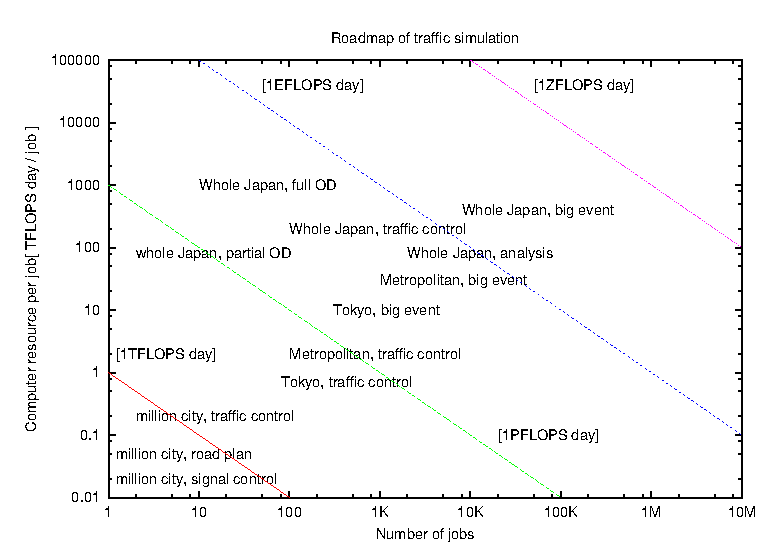
\includegraphics[width=9cm,keepaspectratio]{research/ito/traffic.eps}

  (2) \includegraphics[width=9cm,keepaspectratio]{research/ito/market.eps}

  (3) \includegraphics[width=9cm,keepaspectratio]{research/ito/evacuation.eps}

\vspace{1cm}

  \caption{Roadmaps of agent-based simulations of (1) car traffic, (2) market and (3) evacuation are plotted.
Horizontal axis shows estimated number of simulation jobs to achieve each task.
Vertical axis shows computer resources of each job in a unit of TFLOPS$\cdot$day, Lines of -45 degree correspond to lines of equal computational effort\cite{NIYMKMYHA}.}
  \locallabel{FIGROADMAP}
\end{figure}



%%% DO NOT EDIT BELOW

\section{Publications}

%\printbibliography[keyword=journal, heading=subbibliography, title={Journal Articles}, prefixnumbers={1-}, resetnumbers=true]
%\printbibliography[keyword=proceedings, heading=subbibliography, title={Conference Papers}, prefixnumbers={2-}, resetnumbers=true]
%\printbibliography[keyword=invited, heading=subbibliography, title={Invited Talks}, prefixnumbers={3-}, resetnumbers=true]
%\printbibliography[keyword=poster, heading=subbibliography, title={Posters and Presentations}, prefixnumbers={4-}, resetnumbers=true]
%\printbibliography[keyword=deliverable, heading=subbibliography, title={Patents and Deliverables}, prefixnumbers={5-}, resetnumbers=true]

\printbibliography[keyword=journal, heading=subbibliography, title={Journal Articles}, resetnumbers=true]
\printbibliography[keyword=proceedings, heading=subbibliography, title={Conference Papers}]
\printbibliography[keyword=invited, heading=subbibliography, title={Invited Talks}]
\printbibliography[keyword=poster, heading=subbibliography, title={Posters and Presentations}]
\printbibliography[keyword=deliverable, heading=subbibliography, title={Patents and Deliverables}]

\end{refsection}
